%\chapterauthor{Author Name}{Author Affiliation}
%\chapterauthor{Second Author}{Second Author Affiliation}
\chapter{Limit} \label{ch1title}

Consider a sequence $\{a_n\}$ or a function $f(x)$. In this chapter, the values of $a_n$ or $f(x)$ when $n$ or $x$ grows towards infinity are discussed. The value of $f(x)$ when $x$ approaches a constant value is discussed.

\section{Limit of Sequence} \label{ch1sec:limitofsequence}

A motivating example of the limit of a sequence is given in Section \ref{ch1subsec:sequencemotivatingexample}. The definition of the limit of a sequence is given in Section \ref{ch1subsec:definationoflimitofsequence}. The calculation of the limit of a sequence is discussed in \ref{chisubsec:proofofsequenceconvergence}, mainly on the proof of convergence of a sequence.

\subsection{Motivating Example} \label{ch1subsec:sequencemotivatingexample}

We use $\{a_n\}$ to denote a \mync{sequence}. In $\{a_n\}$, the positive integer $n$ is the index of the elements in the sequence, where $a_1$ represents the first element of $\{a_n\}$, and $a_2$ the second element, and so on. A sequence has at least one element $a_1$. It may have finite elements, in which case it is called a \mync{finite sequence}. Or, it may have infinite elements, in which case it is called an \mync{infinite sequence}. In this notebook, we are mostly interested in infinite sequences.

A motivating example is given below to illustrate the limit of an infinite sequence.

\begin{shortbox}
\Boxhead{A Motivating Example}

Consider an infinite sequence $\{a_n\}$ whose elements are recursively calculated by
\begin{eqnarray}
  a_1 &=& 1, \label{ch1eq:motivatingexampleinitialcondition} \\
  a_n &=& a_{n-1} + \left(\dfrac{1}{2}\right)^{n-1}. \label{ch1eq:motivatingexamplerecursive}
\end{eqnarray}

Q1: Calculate the feasible domain of $n$ such that $a_n\geq 1.95$.

Q2: Calculate the feasible domain of $n$ such that $a_n\geq 2$.
\end{shortbox}

The old school way of solving the questions is rather simple: use a table to list down different $n$ and its corresponding $a_n$. The value of $a_n$ can be manually calculated for small $n$, as shown in Table \ref{chi1table:smallan}. In theory, this table can be extended to any $n$ of choice. From Table \ref{chi1table:smallan}, for any $n\geq6$, $a_n \geq 1.95$.

\begin{table}[ht]
\tabletitle{Calculate $a_n$ for any arbitrary $n$ in the motivating example.} \label{chi1table:smallan}
\begin{tabular}{lll}
\tch{$n$}    &\tch{$a_n - a_{n-1}=\left(\dfrac{1}{2}\right)^{n-1}$} &\tch{$a_n$} \\ \hline
$1$ & --- & $1$ \\
$2$ & $0.5$ & $1.5$ \\
$3$ & $0.25$ & $1.75$ \\
$4$ & $0.125$ & $1.875$ \\
$5$ & $0.0625$ & $1.9375$ \\
$6$ & $0.03125$ & $1.96875$ \\
$7$ & $0.015625$ & $1.984375$ \\
$\vdots$ & $\vdots$ & $\vdots$ \\ \hline
\end{tabular}
\end{table}

To find out the feasible range of $n$ such that $a_n \geq 2$, we can start by investigating a larger table, say Table \ref{chi1table:largean}. From Table \ref{chi1table:largean}, it can been seen that as $n$ grows larger and larger, the increment $a_n - a_{n-1} = \left(\dfrac{1}{2}\right)^{n-1}$ becomes smaller and smaller, and the increment is just hardly enough to top $a_n$ to $2$.

\begin{table}[ht]
\tabletitle{Calculate $a_n$ for any arbitrary $n$ in the motivating example, but longer table.} \label{chi1table:largean}
\begin{tabular}{lll}
\tch{$n$}    &\tch{$a_n - a_{n-1}=\left(\dfrac{1}{2}\right)^{n-1}$} &\tch{$a_n$} \\ \hline
$1$ & $1$ & $1$ \\
$2$ & $0.5$ & $1.5$ \\
$3$ & $0.25$ & $1.75$ \\
$4$ & $0.125$ & $1.875$ \\
$5$ & $0.0625$ & $1.9375$ \\
$6$ & $0.03125$ & $1.96875$ \\
$7$ & $0.015625$ & $1.984375$ \\
$8$ & $0.0078125$ & $1.9921875$ \\
$9$ & $0.00390625$ & $1.99609375$ \\
$10$ & $0.001953125$ & $1.998046875$ \\
$11$ & $0.0009765625$ & $1.9990234375$ \\
$12$ & $0.00048828125$ & $1.99951171875$ \\
$13$ & $0.000244140625$ & $1.999755859375$ \\
$14$ & $0.0001220703125$ & $1.9998779296875$ \\
$15$ & $0.00006103515625$ & $1.99993896484375$ \\
$\vdots$ & $\vdots$ & $\vdots$ \\ \hline
\end{tabular}
\end{table}

An alternative method to find the feasible range is to derive an analytical equation of $a_n$ as a function of $n$, and we can solve $a_n\geq 2$ for $n$. Recursively using \eqref{ch1eq:motivatingexamplerecursive} for $t-1$ times and substituting \eqref{ch1eq:motivatingexampleinitialcondition} into \eqref{ch1eq:motivatingexamplerecursive} give
\begin{eqnarray}
  a_n &=& \sum_{i=1}^{n} \left(\dfrac{1}{2}\right)^{i-1} \label{eq:ch1:analyticalv} \\
  &=& 1 + \sum_{i=2}^{n} \left(\dfrac{1}{2}\right)^{i-1}, \label{eq:ch1:analyticalv2}
\end{eqnarray}
and from \eqref{eq:ch1:analyticalv}
\begin{eqnarray}
  \dfrac{1}{2}a_n &=& \sum_{i=1}^{n} \left(\dfrac{1}{2}\right)^{i} \nonumber \\
  &=& \sum_{i=2}^{n} \left(\dfrac{1}{2}\right)^{i-1} + \left(\dfrac{1}{2}\right)^{n}. \label{eq:ch1:analyticalhalfv}
\end{eqnarray}
Subtracting \eqref{eq:ch1:analyticalhalfv} from \eqref{eq:ch1:analyticalv2} gives
\begin{eqnarray}
  \dfrac{1}{2}a_n &=& 1 - \left(\dfrac{1}{2}\right)^{n}, \nonumber \\
  a_n &=& 2 - \left(\dfrac{1}{2}\right)^{n-1}. \label{eq:ch1:analyticalvresult}
\end{eqnarray}

Equation \eqref{eq:ch1:analyticalvresult} can be verified using the results in Table \ref{chi1table:largean}. It suggests that the elements in sequence $\{a_n\}$ will never reach 2 for any $n$, although $a_n$ can be very close to $2$ as $n$ increases. This can also be shown from the plot of \eqref{eq:ch1:analyticalvresult} as given in Fig. \ref{ch1fig:motivatingexp}.
\begin{figure}
\centering
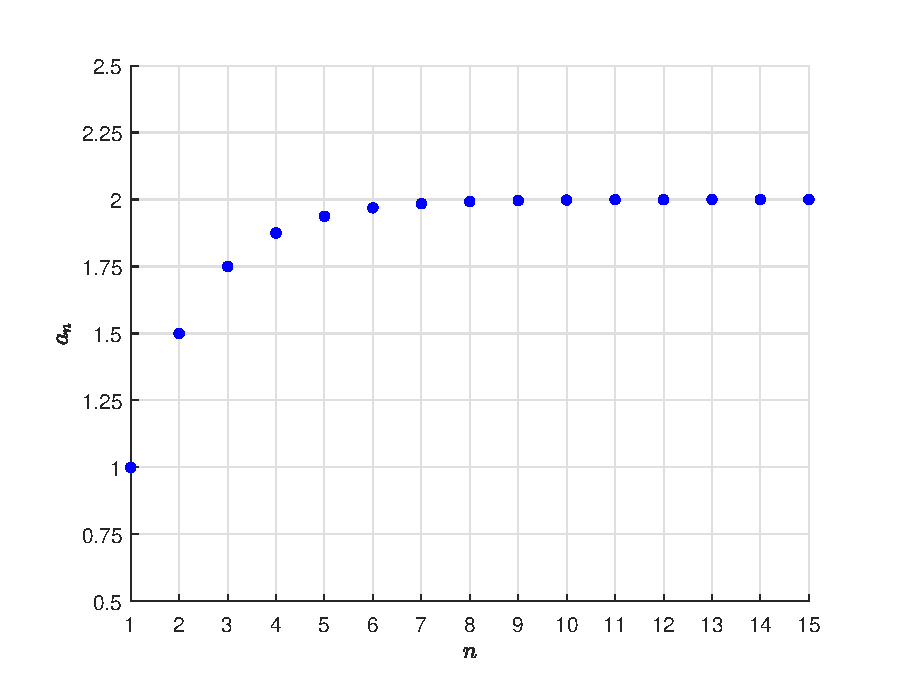
\includegraphics[width=250pt]{chapters/part-1/figures/fig_motivatingexp.eps}
\caption{Plot of $a_n$ as a function of $n$ in the motivating example. The readings of $a_n$ are given in Table \ref{chi1table:largean}.} \label{ch1fig:motivatingexp}
\end{figure}

The following features can be observed for sequence $\{a_n\}$ from both \eqref{eq:ch1:analyticalvresult} and Fig. \ref{ch1fig:motivatingexp}.
\begin{itemize}
  \item The sequence is monotonically increasing, as $a_{n-1}<a_n$ for any $n$.
  \item The sequence is bounded, as $a_n<2$ for any $n$.
  \item The sequence can get ``as close to $2$ as we like'', in the sense that for any value smaller than 2, however close to 2 it is (say, 1.9999), $a_n$ will at some point exceeds that value and get even closer to 2, for large enough $n$.
\end{itemize}

Sequence $\{a_n\}$ reveals an important but not intuitive fact: it is possible to find a monotonically increasing yet bounded sequence. Another way to look at it is that it is possible to add infinite number of positive values together, yet the result is a finite value. From the fact that $\{a_n\}$ gets as close to a certain value as possible when $n$ gets large enough, the limit of sequence is defined, as introduced in the next Section \ref{ch1subsec:definationoflimitofsequence}.

\subsection{Limit of Sequence} \label{ch1subsec:definationoflimitofsequence}

Given an infinite sequence $\{a_n\}$, if $\{a_n\}$ is bounded and it gets close to a value $L$ ``as close as we like'' for large $n$, then $L$ is called the \mync{limit of the sequence}. The formal definition of the limit of a sequence is given below.

\begin{VF}
\textbf{Definition of the limit of sequence}:
\\
\\
\noindent A sequence $\{a_n\}$ has limit $L$ if for any $\varepsilon > 0$ (however small it is), there is always a corresponding integer $N$, such that if $n>N$, $|a_n-L|<\varepsilon$. This is denoted by
\begin{eqnarray}
  \lim_{n\rightarrow \infty} a_n &=& L, \nonumber
\end{eqnarray}
or
\begin{eqnarray}
  a_n \rightarrow L  & \textup{as} & n \rightarrow \infty, \nonumber
\end{eqnarray}
and in this case we say ``sequence $\{a_n\}$ is convergent'' and ``sequence $\{a_n\}$ converges to $L$ (as $n$ approaches infinity)''.
\end{VF}

If an infinite sequence has a limit, it is known as a \mync{convergent sequence}. Otherwise, it is known as a \mync{divergent sequence}. The sequence $\{a_n\}$ in \eqref{eq:ch1:analyticalvresult} is an example of a convergent sequence that converges to $2$. We can easily prove this using the definition of the limit of a sequence as follows.

Given any $\varepsilon > 0$, from \eqref{eq:ch1:analyticalvresult} solving
\begin{eqnarray}
  |a_n - 2| &<& \varepsilon \nonumber
\end{eqnarray}
gives
\begin{eqnarray}
  \left|2-\left(\dfrac{1}{2}\right)^{n-1}-2\right| &<& \varepsilon, \nonumber \\
  n &>& 1-\textup{log}_2\varepsilon. \label{eq:ch1:motivatingexamplenrange}
\end{eqnarray}
As long as $N$ is an integer satisfying $N > 1-\textup{log}_2\varepsilon$, for $n > N$, $|a_n - 2| < \varepsilon$ can be achieved. For example, if $\varepsilon = 0.05$, \eqref{eq:ch1:motivatingexamplenrange} gives $n>5.32$. This implies that by letting $N = 6$ (or $7$, $8$, ...), for any $n \geq N$, $|a_n-2|<0.05$. This matches the observation given in Table \ref{chi1table:smallan}.

If there is no such limit $L$ for an infinite sequence $\{a_n\}$, we say ``sequence $\{a_n\}$ is divergent'' or ``sequence $\{a_n\}$ diverges''.

As a special case of divergent sequences, if $\{a_n\}$ becomes unbounded as $n$ approaches infinity, we say ``sequence $\{a_n\}$ diverges to infinity''. The definition is as follows.
\begin{VF}
\textbf{Definition of sequence diverging to infinity}:
\\
\\
\noindent For a sequence $\{a_n\}$, if for any arbitrary positive value $M$ (however large it is), there is always a corresponding integer $N$, such that if $n>N$, $|a_n|>M$, we say ``$\{a_n\}$ diverges to infinity''. This is denote it by
\begin{eqnarray}
  \lim_{n\rightarrow \infty}a_n &=& \infty. \nonumber
\end{eqnarray}
\end{VF}

Sequence $\{s_n\}$ where $s_n=\sum_{i=1}^{n}a_n$ is used to denote the sum of the first $n$ elements in the infinite sequence $\{a_n\}$. Apparently, for infinite sequence $\{a_n\}$, $\{s_n\}$ is also an infinite sequence which may or may not converge depending on $\{a_n\}$. The limit of $\{s_n\}$ is denoted by
\begin{eqnarray}
  \lim_{n\rightarrow\infty}s_n &=& \sum_{i=1}^{\infty} a_n \nonumber
\end{eqnarray}
if $\{s_n\}$ converges and $\sum_{i=1}^{\infty} a_n$ exists. Otherwise, $\{s_n\}$ diverges and $\sum_{i=1}^{\infty} a_n$ does not exist.

\subsection{Calculation of the Limit of a Sequence} \label{chisubsec:proofofsequenceconvergence}

As the first step in the calculation of the limit of a sequence, the convergence of the sequence must be proved. It makes no sense to calculate the limit if it does not exist in the first place. This section mainly focuses on the proof of convergence of a sequence. Usually, after proving the convergence, the limit can be obtained by either using numerical methods or calculating the limit of the function $a_n=f(n)$ as a function of $n$. More details of calculating the limit of a function are given in Section \ref{ch1sec:limitofafunction}.

Generally speaking, there is no systematic way of proving the convergence or divergence of an infinite sequence except using the definition. Sometimes the proof can be very difficult or even impossible. Some well-studied and commonly seen sequences are summarized in the following Table \ref{chi1table:sequencexample}.
\begin{table}[!htb]
\caption{Convergence of commonly seen $\{a_n\}$ and $\{s_n\}$. Variable $c$, $r$ are constants.} \label{chi1table:sequencexample}
\begin{tabular}{lllcc}\hline
\tch{Category} & \tch{$a_n$} & \tch{$s_n$} & $\lim_{n\rightarrow\infty}a_n$ & $\lim_{n\rightarrow\infty}s_n$ \\ \hline
Polynomial & $c$, $c\neq 0$ & $nc$ & c & $\infty$ \\
& $n$ & $\dfrac{n(n+1)}{2}$ & $\infty$ & $\infty$ \\
& $n^2$ & $\dfrac{n(n+1)(2n+1)}{6}$ & $\infty$ & $\infty$ \\
& $n^3$ & $\dfrac{n^2(n+1)^2}{4}$ & $\infty$ & $\infty$ \\
Power Series & $cr^{n-1}, |r|<1$ & $\dfrac{c(1-r^n)}{1-r}$ & $0$ & $\dfrac{c}{1-r}$ \\
Others & $n^{-1}$ & --- & $0$ & $\infty$ \\
& $n^{-2}$ & --- & $0$ & $\dfrac{\pi}{6}$ \\ \hline
\end{tabular}
\footnotesize{``$\infty$'' stands for ``diverges to infinity''.}
\end{table}

If a sequence falls into one of the above categories, or somewhat similar to the above categories, or can be expressed as a compound sequence derived from the above categories, its convergence or divergence might be proved a bit easier. For example, if $c_n = a_n + b_n$, and both ${a_n}$ and ${b_n}$ converge, then
\begin{eqnarray}
  \lim_{n \rightarrow \infty}c_n &=& \lim_{n \rightarrow \infty}a_n + \lim_{n \rightarrow \infty}b_n. \nonumber
\end{eqnarray} This can be proved using the definition of the limitation of the sequence.

Some other interesting features regarding sequence convergence are given as follows. Given two sequences $\{a_n\}$ and $\{b_n\}$, if
\begin{eqnarray}
  \lim_{n\rightarrow\infty} \dfrac{a_n}{b_n} = L \neq 0, \nonumber
\end{eqnarray}
then $\{a_n\}$ and $\{b_n\}$ must behave the same in terms of convergence, meaning that both of them must converge or diverge at the same time.

It is intuitive and not difficult to prove that for $\{s_n\}$ to converge, i.e. $\lim_{n\rightarrow\infty}s_n = s$, it is necessary (but not sufficient) for its corresponding $\{a_n\}$ to converge to zero, i.e. $\lim_{n\rightarrow\infty}a_n = 0$. Do notice that it is possible to have a divergent $\{s_n\}$ even if $a_n$ converges to zero. An example is the harmonic series given in Table \ref{chi1table:sequencexample} where $a_n = n^{-1}$. 

The famous \mync{monotone convergence theorem for sequence} given below can become handy when proving the convergence of a sequence.
\begin{VF}
\textbf{Monotone Convergence Theorem for Sequence}:
\\
\\
\noindent If a sequence $\{a_n\}$ is monotonically increasing or decreasing, and meantime it is bounded, i.e. $|a_n| < M$ for all $n$, then $\{a_n\}$ must be convergent
\end{VF}
The proof of this theorem is not included in this notebook.

From the monotone convergence theorem, we know that for a sequence $\{a_n\}$, if $\sum_{i=1}^{\infty}|a_n|$ exists, then the infinite sum $\sum_{i=1}^{\infty}a_n$ must also exist. This can be illustrated simply by splitting $\{a_n\}$ into $\{a_n^+\}$ and $\{a_n^-\}$, where
\begin{eqnarray}
  a_n^+ &=& \left\{\begin{array}{cc}
                     a_n & a_n \geq 0 \\
                     0 & a_n < 0
                   \end{array}\right.,  \nonumber \\
  a_n^- &=& \left\{\begin{array}{cc}
                     -a_n & a_n < 0 \\
                     0 & a_n \geq 0
                   \end{array}\right.. \nonumber
\end{eqnarray}
Apparently, both $a_n^+$ and $a_n^-$ are non-negative. Therefore, both $\sum_na_n^+$ and $\sum_na_n^-$ are monotonically increasing non-negative sequences. We also know that both of them are bounded because $\sum_{n}|a_n| = \sum_{n}a_n^+ + \sum_{n}a_n^-$ is bounded. Therefore, both $\sum_na_n^+$ and $\sum_na_n^-$ must be convergent according to the monotone convergence theorem. This implies that $\sum a_n = \sum a_n^+ - \sum a_n^-$ must also be a convergent sequence as it is the sum of two convergent sequences.

Sequence $a_n$ with bounded $\sum_{i=1}^{\infty}|a_n|$ is known as an \mync{absolutely convergent sequence}. An absolutely convergent sequence $a_n$ must have a bounded infinite sum $\sum_{i=1}^{\infty}a_n$, but might not be true wise versa.

\section{Limit of Function} \label{ch1sec:limitofafunction}

A motivating example is given in Section \ref{ch1subsec:functionmotivatingexample}. The definition of the limit of a function is given in Section \ref{ch1subsec:definationoflimitoffunction}. The calculation of the limit of a function is discussed in \ref{ch1subsec:calculationlimitfunction}.

\subsection{Motivating Example} \label{ch1subsec:functionmotivatingexample}

A motivating example is given below to illustrate the limit of a function.

\begin{shortbox}
\Boxhead{A Motivating Example}

Consider function
\begin{eqnarray}
  y = f(x) = \left\{\begin{array}{cc}
                    (x-1)^2 & x \neq 1 \\
                    1 & x = 1
                  \end{array}\right.. \label{ch1eq:fxsimple}
\end{eqnarray}

Q1: Obtain the domain for $x$ and range for $y$.

Q2: Calculate $y$ at $x = 1$.

Q3: Calculate $y$ when $x$ is in a small ``neighbourhood'' of $1$, but $x \neq 1$.

\end{shortbox}

For Q1, the plot of $y$ as a function of $x$ is given in Fig \ref{ch1fig:fxsimpleexample}. It is clear from the figure that the domain and range of the function are $x\in \mathbb{R}$ and $y\in \mathbb{R}, y > 0$ respectively. For Q2, substituting $x=1$ into \eqref{ch1eq:fxsimple} gives $y=1$, as it is also shown in Fig \ref{ch1fig:fxsimpleexample}.

\begin{figure}
\centering
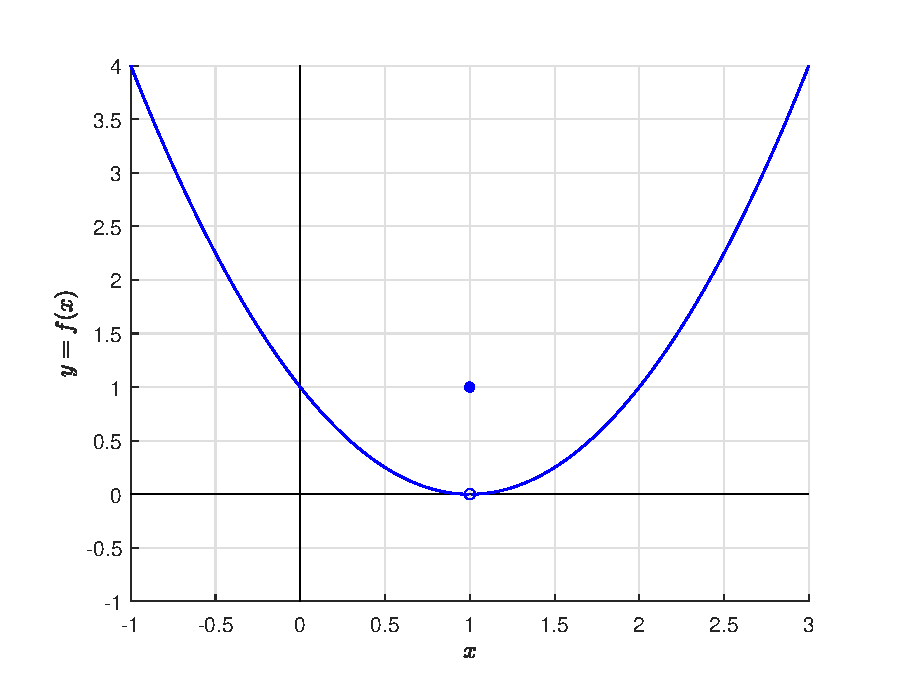
\includegraphics[width=250pt]{chapters/part-1/figures/fig_fxsimple.eps}
\caption{Plot of $y$ as a function of $x$ in the motivating example.} \label{ch1fig:fxsimpleexample}
\end{figure}

For Q3, we need to rewrite ``$x$ is in a small neighbourhood of $1$, but $x \neq 1$'' in a bit more precise manner. An intuitive way is to define a small ``threshold area'' near $x=1$, say, $-\delta < x-1 < \delta, x \neq 1$ with $\delta$ being a very small positive value. Notice that $x=1$ is not concerned and the value of $y$ near $x=1$ has nothing to do with $y$ at $x=1$.

Next, we can calculate $y$ subject to $-\delta < x-1 < \delta, x \neq 1$. Clearly, the range of $y$ relates to the choice of $\delta$. Substituting $-\delta < x-1 < \delta, x \neq 1$ into \eqref{ch1eq:fxsimple} gives $0 < y < \delta^2$. With $\delta$ being chosen smaller and smaller, the range of $y$ would become smaller and smaller, and $y$ will eventually approach $0$ (although $y$ cannot be precisely $0$).

This discussion is essentially a study of $y$ when $x$ is ``as close as we like but not equal'' to $1$. We have learned that in this motivating example:
\begin{itemize}
  \item The value of $y$ when $x$ is ``as close as we like to $1$'' does not rely on the value of $y$ at $x = 1$.
  \item The value of $y$ when $x$ is ``as close as we like to $1$'' floats in a small range depending on the size of the ``neighbourhood'' of $1$ where $x$ residents. The size of the ``neighbourhood'' is quantified by $\delta$ in this example. Thus, the range of $y$ is related to the choice of $\delta$.
  \item With a proper choice of $\delta$, the value of $y$ can be as ``close as we like to $0$''.
\end{itemize}
The above features give a brief idea of limit of a function. In the example, $y$ can be made as close as we like to $0$ simply by making $x$ close enough to $1$ by choosing a small $\delta$.

\subsection{Limit of a Function} \label{ch1subsec:definationoflimitoffunction}

The formal definition of the \mync{limit of the function} is given below. Notice that there are a few different but equivalent ways to define the limit of a function. Here the ``$\varepsilon$-$\delta$ definition'' is introduced.

\begin{VF}
\textbf{Definition of the limit of the function at $x\rightarrow a$}:
\\
\\
\noindent A function $f(x)$ of $x$ has the limit $L$ at $x=a$ if for any $\varepsilon > 0$, there is always a corresponding $\delta > 0$, such that if $0<|x-a|<\delta$, $|f(x)-L| < \varepsilon$, with the prerequisite that $0<|x-a|<\delta$ is defined for $f(x)$. This is denoted by
\begin{eqnarray}
   \lim_{x\rightarrow a} f(x) &=& L, \nonumber
\end{eqnarray}
or
\begin{eqnarray}
  f(x) \rightarrow L & \textup{as} & x \rightarrow a. \nonumber
\end{eqnarray}
\end{VF}

Using the definition above, it can be proved easily that for the motivating example in Section \ref{ch1subsec:functionmotivatingexample}, the function $y=f(x)$ has a limit of $\lim_{x\rightarrow 1}f(x)=0$. Notice that $\lim_{x\rightarrow a}f(x)=L$ does not necessarily require $f(a)=L$. As a matter of fact, $f(x)$ does not even need to be defined at $x=a$, as long as it is defined at the neighbour of $x=a$.

Similar to the definition of the limit of a function, the definition of \mync{one-sided limit of the function} is given below. The one-sided limit is similar but weaker than the definition of the limit of a function in the sense that it only concerns one side of the neighbour of $x=a$.

\begin{VF}
\textbf{Definition of the one-sided limit of the function}:
\\
\\
\noindent A function $f(x)$ of $x$ has the one-side left limit $L^-$ at $x=a$ if for any $\varepsilon > 0$, there is always a corresponding $\delta > 0$, such that if $a-\delta<x<a$, $|f(x)-L^-| < \varepsilon$, with prerequisite that $a-\delta<x<a$ is defined for $f(x)$. This is denoted by
\begin{eqnarray}
   \lim_{x\rightarrow a^-} f(x) &=& L^-, \nonumber
\end{eqnarray}
or
\begin{eqnarray}
  f(x) \rightarrow L^- & \textup{as} & x \rightarrow a^-. \nonumber
\end{eqnarray}
\\
\\
\noindent A function $f(x)$ of $x$ has the one-side right limit $L^+$ at $x=a$ if for any $\varepsilon > 0$, there is always a corresponding $\delta > 0$, such that if $a<x<a+\delta$, $|f(x)-L^+| < \varepsilon$, with prerequisite that $a<x<a+\delta$ is defined for $f(x)$. This is denoted by
\begin{eqnarray}
   \lim_{x\rightarrow a^+} f(x) &=& L^+, \nonumber
\end{eqnarray}
or
\begin{eqnarray}
  f(x) \rightarrow L^+ & \textup{as} & x \rightarrow a^+. \nonumber
\end{eqnarray}
\end{VF}

It is clear from the definition that a function $f(x)$ has a limit of $L$ at $x=a$ if and only if it has both one-sided left limit $L^-$ and one-sided right limit $L^+$ at $x=a$ and $L^-=L^+=L$, i.e.
\begin{eqnarray}
  \lim_{x\rightarrow a}f(x)=L &\Leftrightarrow& \lim_{x\rightarrow a^-}f(x) = \lim_{x\rightarrow a^+}f(x) = L. \nonumber
\end{eqnarray}

Furthermore, if function $f(x)$ has a limit $L$ at $x=a$, and also $f(x)=L$, the function $f(x)$ is called a \mync{continuous function at $x=a$}. The example given in the motivating example in Section \ref{ch1subsec:functionmotivatingexample} is not continuous at $x=1$ as $\lim_{x\rightarrow 1}=0$ while $\left.f(x)\right|_{x=1}=1$, which can be seen from Fig. \ref{ch1fig:fxsimpleexample}. However, it is continuous everywhere else. For instance, at $x=0$, $\lim_{x\rightarrow 0}=1$ and $\left.f(x)\right|_{x=0}=1$.

The definition of the limit of a function $f(x)$ when $x$ approaches infinity is given below. It is quite similar to the definition of the limit of an infinite sequence.
\begin{VF}
\textbf{Definition of the limit of the function at $x\rightarrow \pm \infty$}:
\\
\\
\noindent A function $f(x)$ of $x$ has the limit $L$ at $x \rightarrow +\infty$ (sometimes denoted as $x \rightarrow \infty$ for simplicity) if for any $\varepsilon > 0$, there is always a corresponding $\delta$, such that if $x > \delta$, $|f(x)-L| < \varepsilon$, with prerequisite that $x > \delta$ is defined for $f(x)$. This is denoted by
\begin{eqnarray}
   \lim_{x\rightarrow +\infty} f(x) &=& L, \nonumber
\end{eqnarray}
or
\begin{eqnarray}
  f(x) \rightarrow L & \textup{as} & x \rightarrow +\infty. \nonumber
\end{eqnarray}
\\
\\
\noindent A function $f(x)$ of $x$ has the limit $L$ at $x \rightarrow -\infty$ if for any $\varepsilon > 0$, there is always a corresponding $\delta$, such that if $x < \delta$, $|f(x)-L| < \varepsilon$, with prerequisite that $x < \delta$ is defined for $f(x)$. This is denoted by
\begin{eqnarray}
   \lim_{x\rightarrow -\infty} f(x) &=& L, \nonumber
\end{eqnarray}
or
\begin{eqnarray}
  f(x) \rightarrow L & \textup{as} & x \rightarrow -\infty. \nonumber
\end{eqnarray}
\end{VF}

In special cases where the function is unbounded, the limit of the function does not exist and we can use $\lim_{x\rightarrow a}f(x) =  \infty$ and $\lim_{x\rightarrow \pm \infty}f(x) = \infty$ to represent the cases.

\subsection{Calculation of the Limit of a Function} \label{ch1subsec:calculationlimitfunction}

The calculation of the limit of many commonly seen elementary functions are often obvious and easy. This is because these functions are often continuous in the domain, and for a continuous function the limit $\lim_{x\rightarrow a}f(x)$ can be obtained by simply substituting $x=a$ into the function. The limit $\lim_{x\rightarrow \infty}f(x)$ might be slightly difficult but mostly can be obtained from the definition.

Some examples are given below in Table \ref{chi1table:limitoffunction}. For the case of rational function, if $p(a) \neq 0$, $\lim_{x\rightarrow a}\dfrac{q(x)}{p(x)} = \dfrac{q(a)}{p(a)}$. If $p(a)=0$, $\lim_{x\rightarrow a}\dfrac{q(x)}{p(x)}$ depends on the order and coefficients of $q(x)$ and $p(x)$ and may not exist. The limit $\lim_{x\rightarrow \infty}\dfrac{q(x)}{p(x)}$ depends on the order and coefficients of $q(x)$ and $p(x)$ and may not exist.


\begin{table}[!htb]
\centering\caption{Limit of commonly seen elementary functions.} \label{chi1table:limitoffunction}
\begin{tabular}{llll}
\hline
Category & \tch{$f(x)$} & \tch{$\lim_{x\rightarrow a}f(x)$} & \tch{$\lim_{x\rightarrow \infty}f(x)$} \\ \hline
Polynomial & $p(x)$ & $p(a)$ & $\infty$ \\
Root & $\sqrt{x}$ & $\sqrt{a}$ for $a>0$ & $\infty$ \\
Rational & $\dfrac{q(x)}{p(x)}$ & depends & depends \\
Trigonometric & $\textup{sin}(x)$, $\textup{cos}(x)$ & $\textup{sin}(a)$, $\textup{cos}(a)$ & No \\
\multirow{2}{*}{Exponential} & \multirow{2}{*}{$e^{-x}$} & \multirow{2}{*}{$e^{-a}$} & $0$ as $x\rightarrow +\infty$ \\
& & & $\infty$ as $x\rightarrow -\infty$ \\
Logarithm & $\textup{log}_e(x)$ & $\textup{log}_e(a)$ for $a>0$ & $\infty$ \\ \hline
\end{tabular}

\begin{flushleft}
\footnotesize
``$\infty$'' stands for ``unbounded''.
\end{flushleft}

\end{table}

It is worth mentioning a few typical cases where a function $f(x)$ does not have a limit and/or is not continuous.

Case 1: function $f(x)$ does not converge at a neighbourhood of $x=a$, thus does not have a one-sided limit. For example, consider
\begin{eqnarray}
  f(x) &=& \textup{sin}\left(\dfrac{1}{x}\right). \nonumber
\end{eqnarray}
The function is defined at $x\in\mathbb{R},x\neq0$, but it does not have a one-sided limit $\lim_{x\rightarrow 0^-}f(x)$ or $\lim_{x\rightarrow 0^+}f(x)$, as when $x\rightarrow0$, function $f(x)$ oscillates, as shown in Fig. \ref{ch1fig:sinoneoverx}.

\begin{figure}
\centering
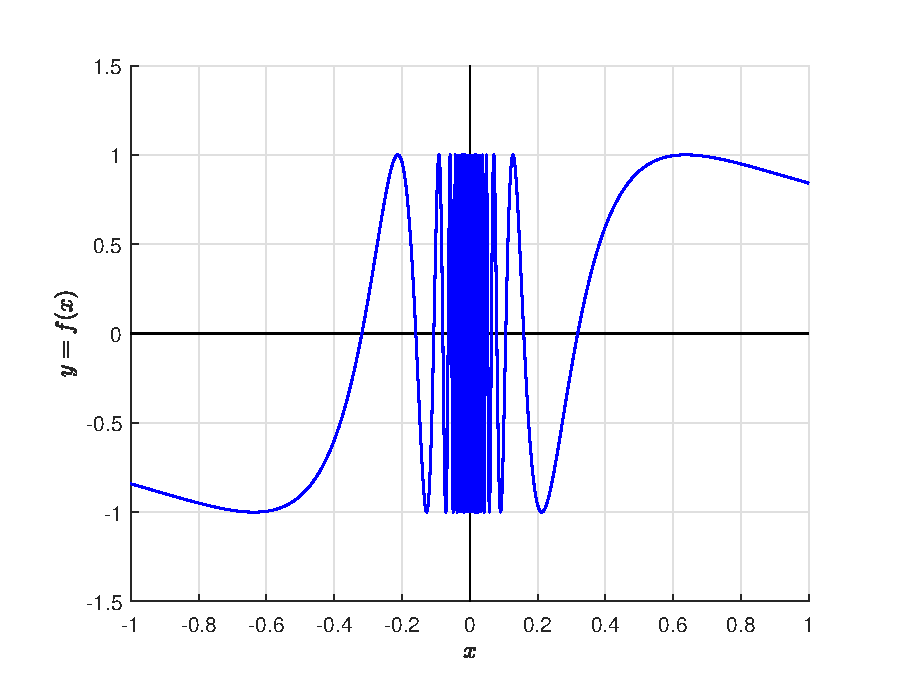
\includegraphics[width=250pt]{chapters/part-1/figures/fig_sinoneoverx.eps}
%%\centerline{\epsfig{/Chapters/chapter1/figures/fig_fxsimple.eps,width=.8\textheight,height=.4\textwidth}}
\caption{Plot of $y=\textup{sin}\left(\dfrac{1}{x}\right)$.} \label{ch1fig:sinoneoverx}
\end{figure}

Case 2: function $f(x)$ is unbounded at a neighbourhood of $x=a$, therefore does not have a one-sided limit. For example, consider
\begin{eqnarray}
  f(x) &=& \left|\dfrac{1}{x}\right|. \nonumber
\end{eqnarray}
Apparently, $\lim_{x\rightarrow 0^-}f(x)$ or $\lim_{x\rightarrow 0^+}f(x)$ does not exist.

Case 3: function $f(x)$ has one-sided limits $\lim_{x\rightarrow 0^-}f(x)$ and $\lim_{x\rightarrow 0^+}f(x)$, but $\lim_{x\rightarrow 0^-}f(x) \neq \lim_{x\rightarrow 0^+}f(x)$. For example, consider
\begin{eqnarray}
  f(x) &=& \textup{sign}(x) = \left\{\begin{array}{cc}
                                    1 & x > 0 \\
                                    0 & x = 0 \\
                                    -1 & x < 0
                                  \end{array}\right..\nonumber
\end{eqnarray}
From the definition, $\lim_{x\rightarrow 0^-}f(x)=-1$ and $\lim_{x\rightarrow 0^+}f(x)=1$, therefore, $\lim_{x\rightarrow 0}f(x)$ does not exist.

Some commonly used tricks are as follows. For $g(x)=f_1(x) + f_2(x)$, if the limits exist for $f_1(x)$ and $f_2(x)$ at $x \rightarrow a$, then
\begin{eqnarray}
  \lim_{x \rightarrow a}g(x) &=& \lim_{x \rightarrow a}f_1(x) + \lim_{x \rightarrow a}f_2(x). \nonumber
\end{eqnarray}
The same is true for the cases $g(x)=f_1(x)f_2(x)$ and $g(x)=\dfrac{f_1(x)}{f_2(x)}$, subject to $\lim_{x \rightarrow a}f_2(x) \neq 0$ when it is the denominator. And it holds true for $x \rightarrow \pm \infty$ as well.

In the case of $g(x)=\dfrac{f_1(x)}{f_2(x)}$ and $\lim_{x \rightarrow a}f_2(x) = 0$, the discussion is more complicated. Sometimes, \textit{L\textprime H\^opital's rule} can become handy. 

\begin{VF}
\textbf{L\textprime H\^opital's rule}:
\\
\\
\noindent For $g(x)=\dfrac{f_1(x)}{f_2(x)}$
\begin{eqnarray}
  g(x) &=& \dfrac{f_1(x)}{f_2(x)} \nonumber
\end{eqnarray}
if the following criteria are satisfied:
\begin{itemize}
  \item Both $\lim_{x\rightarrow a}f_1(x) = 0$ and $\lim_{x\rightarrow a}f_2(x) = 0$.
  \item Both $f_1(x)$, $f_2(x)$ are continuous and differentiable at $x=a$.
  \item The derivative of the denominator $\lim_{x\rightarrow a}f_2^\prime(x) \neq 0$.
\end{itemize}
then $\lim_{x\rightarrow a}g(x)$ can be calculated using \eqref{ch1eq:lhopital}, provided that the right side of \eqref{ch1eq:lhopital} exists.
\begin{eqnarray}
  \lim_{x\rightarrow a}g(x) = \lim_{x\rightarrow a} \dfrac{f_1^\prime(x)}{f_2^\prime(x)}. \label{ch1eq:lhopital}
\end{eqnarray}
where $f^\prime(x)$ is the derivative of $f(x)$.
\end{VF}

The derivative of a function $f(x)$ will be introduced in the next Chapter \ref{ch:derivative}. The proof of L\textprime H\^opital's rule requires solid calculus foundation and is out of the scope of this notebook.

The limit of an infinite sequence is linked to the limit of the associated function at $x\rightarrow\infty$. For example, for sequence $\left\{a_n\right\}$, if $a_n=f(n)$ and $\lim_{n\rightarrow\infty}f(n)=L$, then $\lim_{n\rightarrow\infty}a_n=L$.
